% ============================================================================
%  Problems: เอกซ์โพเนนเชียลและลอการิทึม (Exponential & Logarithmic Functions)
%  Ordered from easy (basic) → intermediate.
%  Shared by exercise.tex and answer-key.tex
% ============================================================================

% --- Part 1: พื้นฐาน (Basic) ---
\examsection{ตอนที่ 1: พื้นฐาน — สมบัติเลขยกกำลังและค่าลอการิทึม}

\problem{
  จงหาค่าของ $2^3 \cdot 2^4 \div 2^5$
}{
  $2^3 \cdot 2^4 = 2^7$ \quad $\rightarrow$ \quad
  $2^7 \div 2^5 = 2^{7-5} = 2^2 = 4$
}

\problem{
  จงหาค่าของ $\log_3 81$
}{
  $3^4 = 81$ \quad ดังนั้น \quad $\log_3 81 = 4$
}

\problem{
  จงหาค่าของ $\log_5 1 + \log_2 16$
}{
  $\log_5 1 = 0$ \quad และ \quad $\log_2 16 = 4$ (เพราะ $2^4=16$)

  รวมกัน $= 0 + 4 = 4$
}

% --- Part 2: การประยุกต์ (Intermediate) ---
\examsection{ตอนที่ 2: การประยุกต์ — สมบัติลอการิทึมและการแก้สมการ}

\problem{
  จงเขียน $\log_2 4 + \log_2 8$ ให้อยู่ในรูปพจน์เดียว
}{
  $\log_2 4 + \log_2 8 = \log_2 (4 \times 8) = \log_2 32 = 5$
}

\problem{
  จงหาค่าของ $\log_3 27^4$ โดยใช้สมบัติของลอการิทึม
}{
  $\log_3 27^4 = 4 \log_3 27 = 4 \times 3 = 12$ \quad ($3^3 = 27$)
}

\problem{
  จงหาค่าของ $\log_4 8$ โดยการเปลี่ยนฐาน
}{
  $\log_4 8 = \dfrac{\log_2 8}{\log_2 4} = \dfrac{3}{2}$
}

\problem{
  จงแก้สมการ $3^{x+2} = 81$
}{
  $3^{x+2} = 3^4$ \quad $\rightarrow$ \quad $x+2 = 4$ \quad $\rightarrow$ \quad $x = 2$
}

\problem{
  จงแก้สมการ $\log_2 (x-3) = 4$
}{
  $x-3 = 2^4 = 16$ \quad $\rightarrow$ \quad $x = 19$

  ตรวจสอบ: $x-3 = 16 > 0$ \quad $\checkmark$
}

% --- Part 3: ระดับ สอวน. (POSN Level) ---
\examsection{ตอนที่ 3: ระดับข้อสอบ สอวน.}

\problem{
  (ข้อสอบจริงปี 66 ข้อ 24)  จงพิจารณาว่า กราฟของฟังก์ชันเอ็กซ์โพเนนเชียลที่ผ่านจุด $(1,2)$ ดังรูป จะตัดกับเส้นตรง $x=2$ ที่พิกัดใด
  \begin{center}
    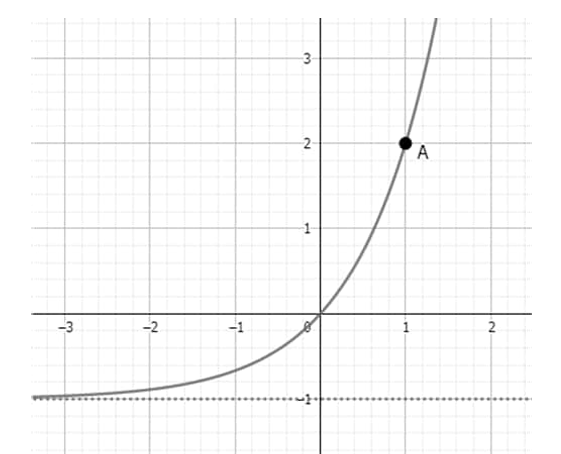
\includegraphics[width=0.5\textwidth]{images/functions-exp-log-01.png}
  \end{center}
}{
  $(2,8)$
}

\problem{
  (ข้อสอบจริงปี 66 ข้อ 22) จงหาผลรวมของคำตอบทั้งหมดของสมการ $6^{\frac{2x-1}{x-1}}-27\cdot  2^{\frac{2x-1}{x-1}} -4\cdot  3^{\frac{2x-1}{x-1}}+108=0$
}{
  $2$
}

\problem{
  (ข้อสอบจริงปี 65 ข้อ 24) ข้อใดเป็นกราฟของ $y=-0.1\ln{x}$ ($\ln$ คือ $\log$ ฐาน $e\approx 2.7$)
  \begin{center}
    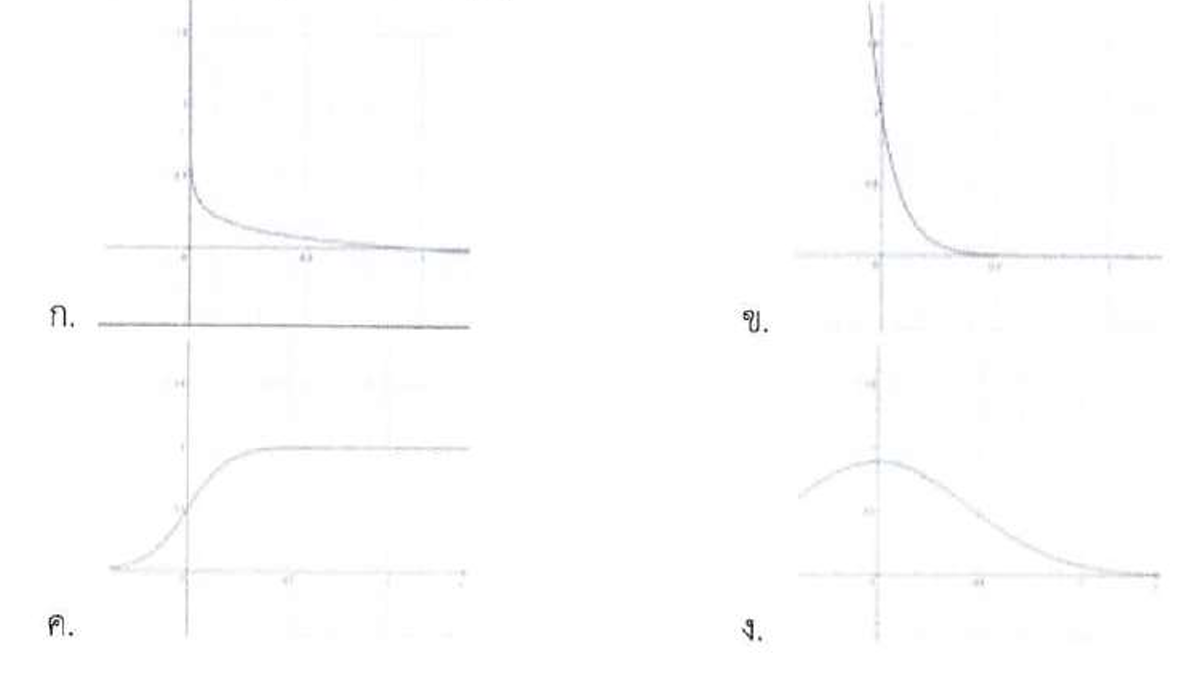
\includegraphics[width=1\textwidth]{images/functions-exp-log-02.png}
  \end{center}
}{
  ก.
}